\documentclass{article}

% Recommended, but optional, packages for figures and better typesetting:
\usepackage{microtype}
\usepackage{graphicx}
\usepackage{subfigure}
\usepackage{booktabs} % for professional tables
\usepackage{color}
\usepackage{enumerate}
% More packages
\usepackage{amsmath, amssymb} %Packages for math symbols 
\usepackage{natbib} % citep
\usepackage{mathtools}
\usepackage{amsthm}
\usepackage{bbm}
\usepackage{multirow}

% hyperref makes hyperlinks in the resulting PDF.
% If your build breaks (sometimes temporarily if a hyperlink spans a page)
% please comment out the following usepackage line and replace
% \usepackage{icml2018} with \usepackage[nohyperref]{icml2018} above.
\usepackage{hyperref}

% Attempt to make hyperref and algorithmic work together better:
\newcommand{\theHalgorithm}{\arabic{algorithm}}
\newcommand{\red}[1]{\textcolor{red}{{#1}}}


\DeclareMathOperator{\argmin}{\arg\min}

% Use the following line for the initial blind version submitted for review:
%\usepackage{icml}
%\usepackage[nohyperref]{icml2018}

% If accepted, instead use the following line for the camera-ready submission:
\usepackage[accepted]{icml2018}

% The \icmltitle you define below is probably too long as a header.
% Therefore, a short form for the running title is supplied here:
\icmltitlerunning{Variable importance via neural networks}

\DeclareMathOperator{\aug}{Aug}
\DeclareMathOperator{\zero}{Zero}
\newtheorem{lemma}{Lemma}

\begin{document}

\twocolumn[
\icmltitle{Supplementary Material to \\
``Nonparametric variable importance\\
           using an augmented neural network with multi-task learning''}

% It is OKAY to include author information, even for blind
% submissions: the style file will automatically remove it for you
% unless you've provided the [accepted] option to the icml2018
% package.

% List of affiliations: The first argument should be a (short)
% identifier you will use later to specify author affiliations
% Academic affiliations should list Department, University, City, Region, Country
% Industry affiliations should list Company, City, Region, Country

% You can specify symbols, otherwise they are numbered in order.
% Ideally, you should not use this facility. Affiliations will be numbered
% in order of appearance and this is the preferred way.
\icmlsetsymbol{equal}{*}

\begin{icmlauthorlist}
\icmlauthor{Jean Feng}{equal,biost}
\icmlauthor{Brian D. Williamson}{equal,biost}
\icmlauthor{Marco Carone}{biost,fhcrc}
\icmlauthor{Noah Simon}{biost}
\end{icmlauthorlist}

\icmlaffiliation{biost}{Department of Biostatistics, University of Washington, Seattle, Washington, USA}
\icmlaffiliation{fhcrc}{Vaccine and Infectious Disease Division, Fred Hutchinson Cancer Research Center, Seattle, Washington, USA}

\icmlcorrespondingauthor{Jean Feng}{jeanfeng@uw.edu}
\icmlcorrespondingauthor{Brian Williamson}{brianw26@uw.edu}

% You may provide any keywords that you
% find helpful for describing your paper; these are used to populate
% the "keywords" metadata in the PDF but will not be shown in the document
\icmlkeywords{Machine Learning, Nonparametric $R^2$, Statistical Inference, Targeted Learning, Variable Importance, Neural Networks}
\vskip 0.3in
]

% this must go after the closing bracket ] following \twocolumn[ ...

% This command actually creates the footnote in the first column
% listing the affiliations and the copyright notice.
% The command takes one argument, which is text to display at the start of the footnote.
% The \icmlEqualContribution command is standard text for equal contribution.
% Remove it (just {}) if you do not need this facility.

%\printAffiliationsAndNotice{}  % leave blank if no need to mention equal contribution
\printAffiliationsAndNotice{\icmlEqualContribution} % otherwise use the standard text.

\section{Proof of Lemma 1}
Using the classic result from \citet{leshno1993multilayer}, we show that there is a neural network that approximates the function $g_{P_0}: \mathbb{R}^p \times \mathbb{R}^p \mapsto \mathbb{R}$ arbitrarily well, where $g_{P_0}$ combines the conditional means into a single function
\begin{align}
\begin{split}
g_{P_0}(x, m) & \coloneqq
\mu_{P_0}(x) \mathbbm{1}\{m = 0\}\\
& + \sum_{s \in \mathcal{S}} \mu_{P_0,s}(x) \mathbbm{1}\{m = e_s\}.
\end{split}
\label{eq:all_conditionals}
\end{align}
Since $g_{P_0}$ contains all the information from the conditional means, such a neural network is also a good approximation of all the conditional means.
\begin{proof}
	For any $\mathcal{S}$, define the augmented conditional function $g_{P_0}(x, m)$ as in \eqref{eq:all_conditionals}.
	Let $\mathcal{E} = \{0\} \cup \{e_s : s \in \mathcal{S}\}$, and let $\tilde{g}_{P_0}(x, m)$ be any continuous function defined over the domain $K \times [-1,2]^{p}$ that shares the same values as $g_{P_0}(x, m)$ over all $K \times \mathcal{E}$.
	Using the result of \citet{leshno1993multilayer}, there exists a sequence of neural networks $\{f_j\}_{j=1}^\infty \in \mathcal{F}$ with parameters $\{\theta_j\}_{j=1}^\infty \in \Theta$ such that
	$$
	\lim_{j\rightarrow\infty}
	\left\|
	f_j \left(x, m; \theta_j \right) - \tilde{g}_{P_0}(x, m)
	\right \|_{L^\infty(K \times [-1,2]^{p})}
	= 0.
	$$
	Our desired result follows from the fact that
	\begin{align*}
	\begin{split}
	&\left\|
	f_j \left(x, m; \theta_j \right) - \tilde{g}_{P_0}(x, m)
	\right \|_{L^\infty(K \times [-1,2]^{p})}\\
	& \ge
	\max_{s \subseteq \mathcal{S}}
	\left\|
	f_j \left(x, e_s; \theta_j \right) - \mu_{P_0, s}(x)
	\right \|_{L^\infty(K)}.
	\end{split}
	\end{align*}
\end{proof}

\section{Experiments on simulated data}\label{sec:sims}

\begin{table*}
\centering
\begin{tabular}{c|l}
& NN structures to cross-validate over\\
\toprule
\multirow{4}{*}{Multiple networks} & Full: 6,40,20,1;6,40,40,1;6,20,20,20,1;6,40,20,20,1 \\
& Reduced $\{x_1, x_2\}$: 4,5,5,1;4,10,5,1; \\
& Reduced $\{x_3, x_4\}$: 4,5,5,1;4,10,5,1; \\
& Reduced $\{x_5, x_6\}$: 4,20,20,20,1;4,40,20,20,1;4,40,40,20,1\\
\hline
Augmented MTL network & 12,40,40,20,1;12,40,40,40,1;12,80,40,40,1 \\
\end{tabular}
\caption{
	Network structures used for multiple networks vs the augmented MTL network in the non-additive six-variable function example.
	The fitting times are similar for fitting a single network (80-200 seconds) since the NN structures used for the two approaches are similar.
	However, there is an increase in time in the multiple networks approach: the practitioner first must spend time finding the correct structures; then, more structures must be cross-validated over, since different covariates have different optimal NN structures.
}
\label{table:timing_experiments}
\end{table*}

\subsection{A non-additive six-variable function}

We consider a situation where $X$ is composed of six features and the conditional mean is a multivariate function that only depends on the first four features:
\begin{align}
f(x_1, ..., x_6) = x_1 \sin(x_1 + 2x_2) \cos(x_3 + 2x_4).
\label{eq:six_func}
\end{align}
We are interested in estimating the variable importance of the groups $\{x_1, x_2\}$, $\{x_3, x_4\}$, and $\{x_5,x_6\}$, given by 0.820, 0.838, and zero, respectively.

In Table \ref{table:timing_experiments}, we display the neural network structures that we cross-validated over to obtain the optimal neural network structure.

\subsection{A sum of univariate functions}

Here we consider the sum of eight univariate functions:
\begin{align}
\begin{split}
f(\boldsymbol{x}) &= x_1 + x_2^2 + \sin(x_3) + \cos(x_4) + (x_5 + 1)^2\\
& - 2x_6 + \max(x_7, 0) + x_8.
\end{split}
\label{eq:eight_additive}
\end{align}
We estimate the importance of all groups with cardinality up to four.

We train the augmented neural network by minimizing the sum of the losses for estimating the full and reduced conditional means:
\begin{align}
\begin{split}
\hat{\theta} &\in \argmin_{\theta \in \Theta^{(2p)}} \frac{1}{n} \sum_{i=1}^n 
\bigg[
\left\{y^{(i)} - f(x^{(i)}, 0; \theta)\right\}^2
\\
&+ \sum_{s \in \mathcal{S}}
\mathbb{E}_{W_s}\left(
\left[y^{(i)} - f(\xi(x^{(i)}, W_s;s), e_s; \theta)\right]^2
\right)
\bigg ],
\end{split}
\label{eq:multi-task-loss}
\end{align}
where $W_s$ is a random variable with value in $\mathbb{R}^{|s|}$; and the function $\xi(x, w; s)$ maps $(x, w)$ to $\mathbb{R}^{p}$ by defining $\{\xi(x, w; s)\}_{(-s)} = x^{(i)}_{(-s)}$ and $\{\xi(x, w; s)\}_s = W_s$.

In Figure \ref{fig:zero_vs_random}, we compare the multi-task loss \eqref{eq:multi-task-loss} when we use 0 for $W_s$ versus when we use a standard normal random variable instead. The minimum loss function value in this setting is 1, due to the variance of the outcome. We see that using random noise results in much improved performance over simply using zero.

\begin{figure}
% AWS: ~/efs/jjfeng/nnet_var_importance/code/_output_fill_zero
% Run python compare_mse_random_v_zero.py
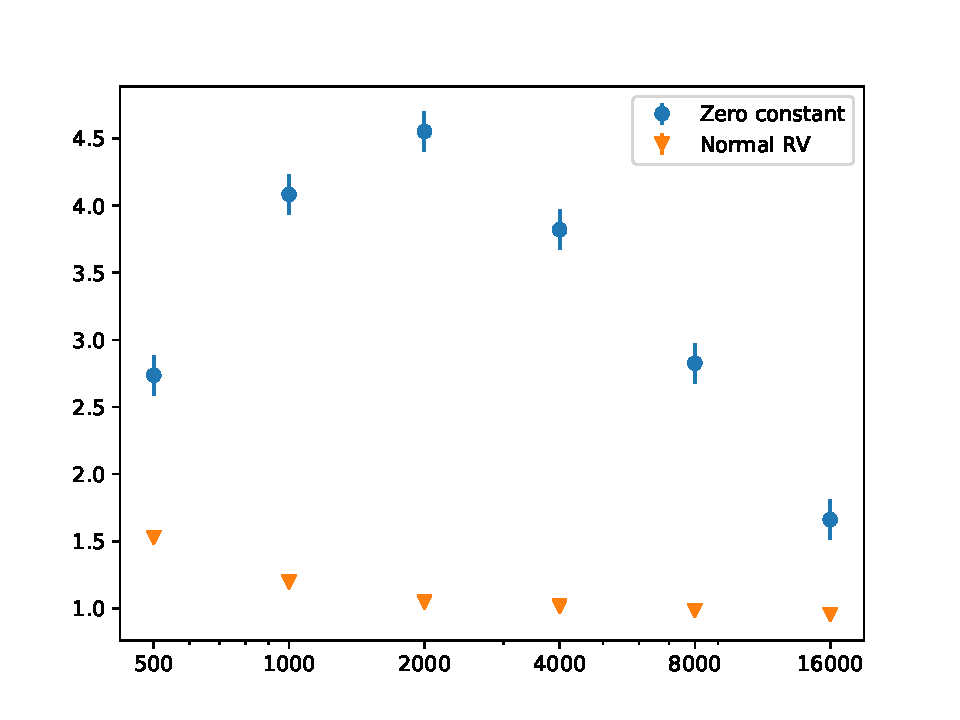
\includegraphics[width=0.4\textwidth]{images/compare_zero_v_random}
\caption{
The multi-task loss \eqref{eq:multi-task-loss} for the simulation specified by \eqref{eq:eight_additive} when fitting MTL augmented networks with $W_s \equiv 0$ vs. $W_s \sim N(0,1)$. The points and error bars represent the mean multi-task loss and its 95\% confidence interval; the errors bars do not show for the normally distributed inputs since the CI is very narrow.
}
\label{fig:zero_vs_random}
\end{figure}

\section{Predicting Mortality of ICU Patients}

%JF Note: someone should probably clean up the language to distinguish between variable, variable groups, features, extracted features, etc. Its a bit confusing.

Here, we analyze the importance of features measured during the first two days of patients' ICU stays for predicting in-hospital mortality using data from Event 1 of the PhysioNet/CinC Challenge 2012 \citep{silva2012predicting}.
The challenge provided a training dataset composed of four thousand records with five general descriptors collected upon admission (gender, age, weight, height, ICU admission type) and 37 features measured over the course of the first 48 hours after admission to the ICU, including the Glasgow Coma Score, blood urea nitrogen, and heart rate, among others.
Some patients never had particular features measured, and some only had them measured once, leading to a large degree of missing data.
%JF I should provide some numbers to show that there is A LOT of missing data in this problem.
Estimating variable importance may provide guidance on which measurements are most informative for predicting in-hospital mortality.

We computed new features based on those proposed in a neural-network submission to the challenge \citep{xia2012neural} and those used to calculate SAPS I and SAPS II scores \citep{le1984simplified, le1993new}.
\citet{xia2012neural} chose to use 18 of the 37 original variables and compute from them a total of 27 features, such as mean, min/max, and the last measurement; their model was then fit on these 27 computed features.
We included these 27 computed features as well as the minimum, maximum, and mean (from fitting linear regression) from the time series of the 18 original variables if they were not already included.
In addition, we (1) added five variables that are used in SAPS I and SAPS II but were not in this set of 18 original variables and (2) included all general descriptors measured at admission.

This procedure resulted in a total of 55 computed and original features in our model (Table~\ref{table:icu_features}).
Though \citet{xia2012neural} did a thorough evaluation to decide which variables to include in the model using univariate classifiers, such classifiers may fail to capture the potentially more complex relationship between the features and mortality; we include a more complete set of features to address this gap, and provide more information by estimating the importance of feature groups.

\begin{table*}
	\begin{center}
\begin{tabular}{c|c|c}
	Variable (Meta)-Group & Variable & Summary (computed or original) \\
	\toprule
	GCS & GCS & last, weighted mean, max, min, slope\\
	\hline
	\multirow{6}{*}{Metabolic panel}  & HCO3 & min, max, last, weighted mean\\
	& BUN & min, max, last, weighted mean\\
	& Na & min, max, weighted mean\\
	& K & min, max, weighted mean\\
	& Glucose & min, max, weighted mean\\
	\hline
	SysABP & SysABP & min, max, last, weighted mean\\
	\hline
	\multirow{2}{*}{CBC} & WBC & min, max, last, weighted mean\\
	& HCT & min, max, weighted mean\\
	\hline
	Temp & Temp & min, max, last, weighted mean\\
	\hline
	Lactate & Lactate & min, max, last, weighted mean \\
	\hline
	HR & HR & min, max, weighted mean\\
	\hline
	\multirow{3}{*}{Respiration} & RespRate & min, max, weighted mean\\
	& MechVent & max \\
	& FiO2, PaO2 & ratio of means\\
	\hline
	Urine & Urine & sum (based on SAPS II urine item)\\
	\hline
	\multirow{5}{*}{General Desc.} & Gender & measured at admission \\
	& Height & measured at admission \\
	& Weight & measured at admission \\
	& Age & measured at admission \\
	& ICU admission type & measured at admission \\
\end{tabular}
	\end{center}
\caption{
Features included for analysis of the PhysioNet/CinC Challenge 2012.
CBC = complete blood count test.
Weighted mean = fit linear regression of response vs. time and get the estimate at the mean measurement time.
Slope = fit linear regression of response vs. time and get slope.
Last = last measurement.
Impossible values were dropped (zero or lower for many of these variables).
}
\label{table:icu_features}
\end{table*}

To understand the importance of running particular tests, we estimate the variable importance of variables grouped by the tests that provide measurements of those variables.
For instance, comprehensive tests like metabolic panels or complete blood counts measure multiple variables.
We group all extracted features for all these variables together as it will help us to understand the importance of running that particular test.
(In addition, those measurements are likely to provide similar information for predicting the response so it would be helpful to relieve that correlation by putting them in a single group -- otherwise we are estimating a ``deflated'' variable importance.)
Thus we estimated the variable importance of groups (first column in Table~\ref{table:icu_features}) as well as individual variables (second column in Table~\ref{table:icu_features}).
Note that individual variables may be extracted into multiple features -- we group these extracted features together to assess the importance of that variable.
Thus we estimate a total of 25 variable importance values.
To estimate variable importance, we fit an augmented network structure with MTL.

As the variables measured across different patients is not always the same, we must handle missing data.
Our method is well-suited for data that is missing at random.
However we expect that many many measurements are not missing at random -- doctors are likely to collect measurements for ones they are concerned about in the patient and ignore collecting measurements that they believe are normal in the patient.
Therefore for features that are likely not to be missing at random, we imputed random values uniformly within the normal ranges of that measurement at each step of stochastic gradient descent.
For features that are likely missing at random, e.g. age, height, weight, we indicated that covariate was missing via the binary augmented/missingness vector and fed in random values for the missing covariate.

We tuned the network structure via training/validation split (80/20) and chose layer sizes 110,4,3,2,1 with relu activation functions for the hidden nodes and a sigmoid function for the output.
The final variable importance estimates are based on models fit on all the data.

\begin{figure}
 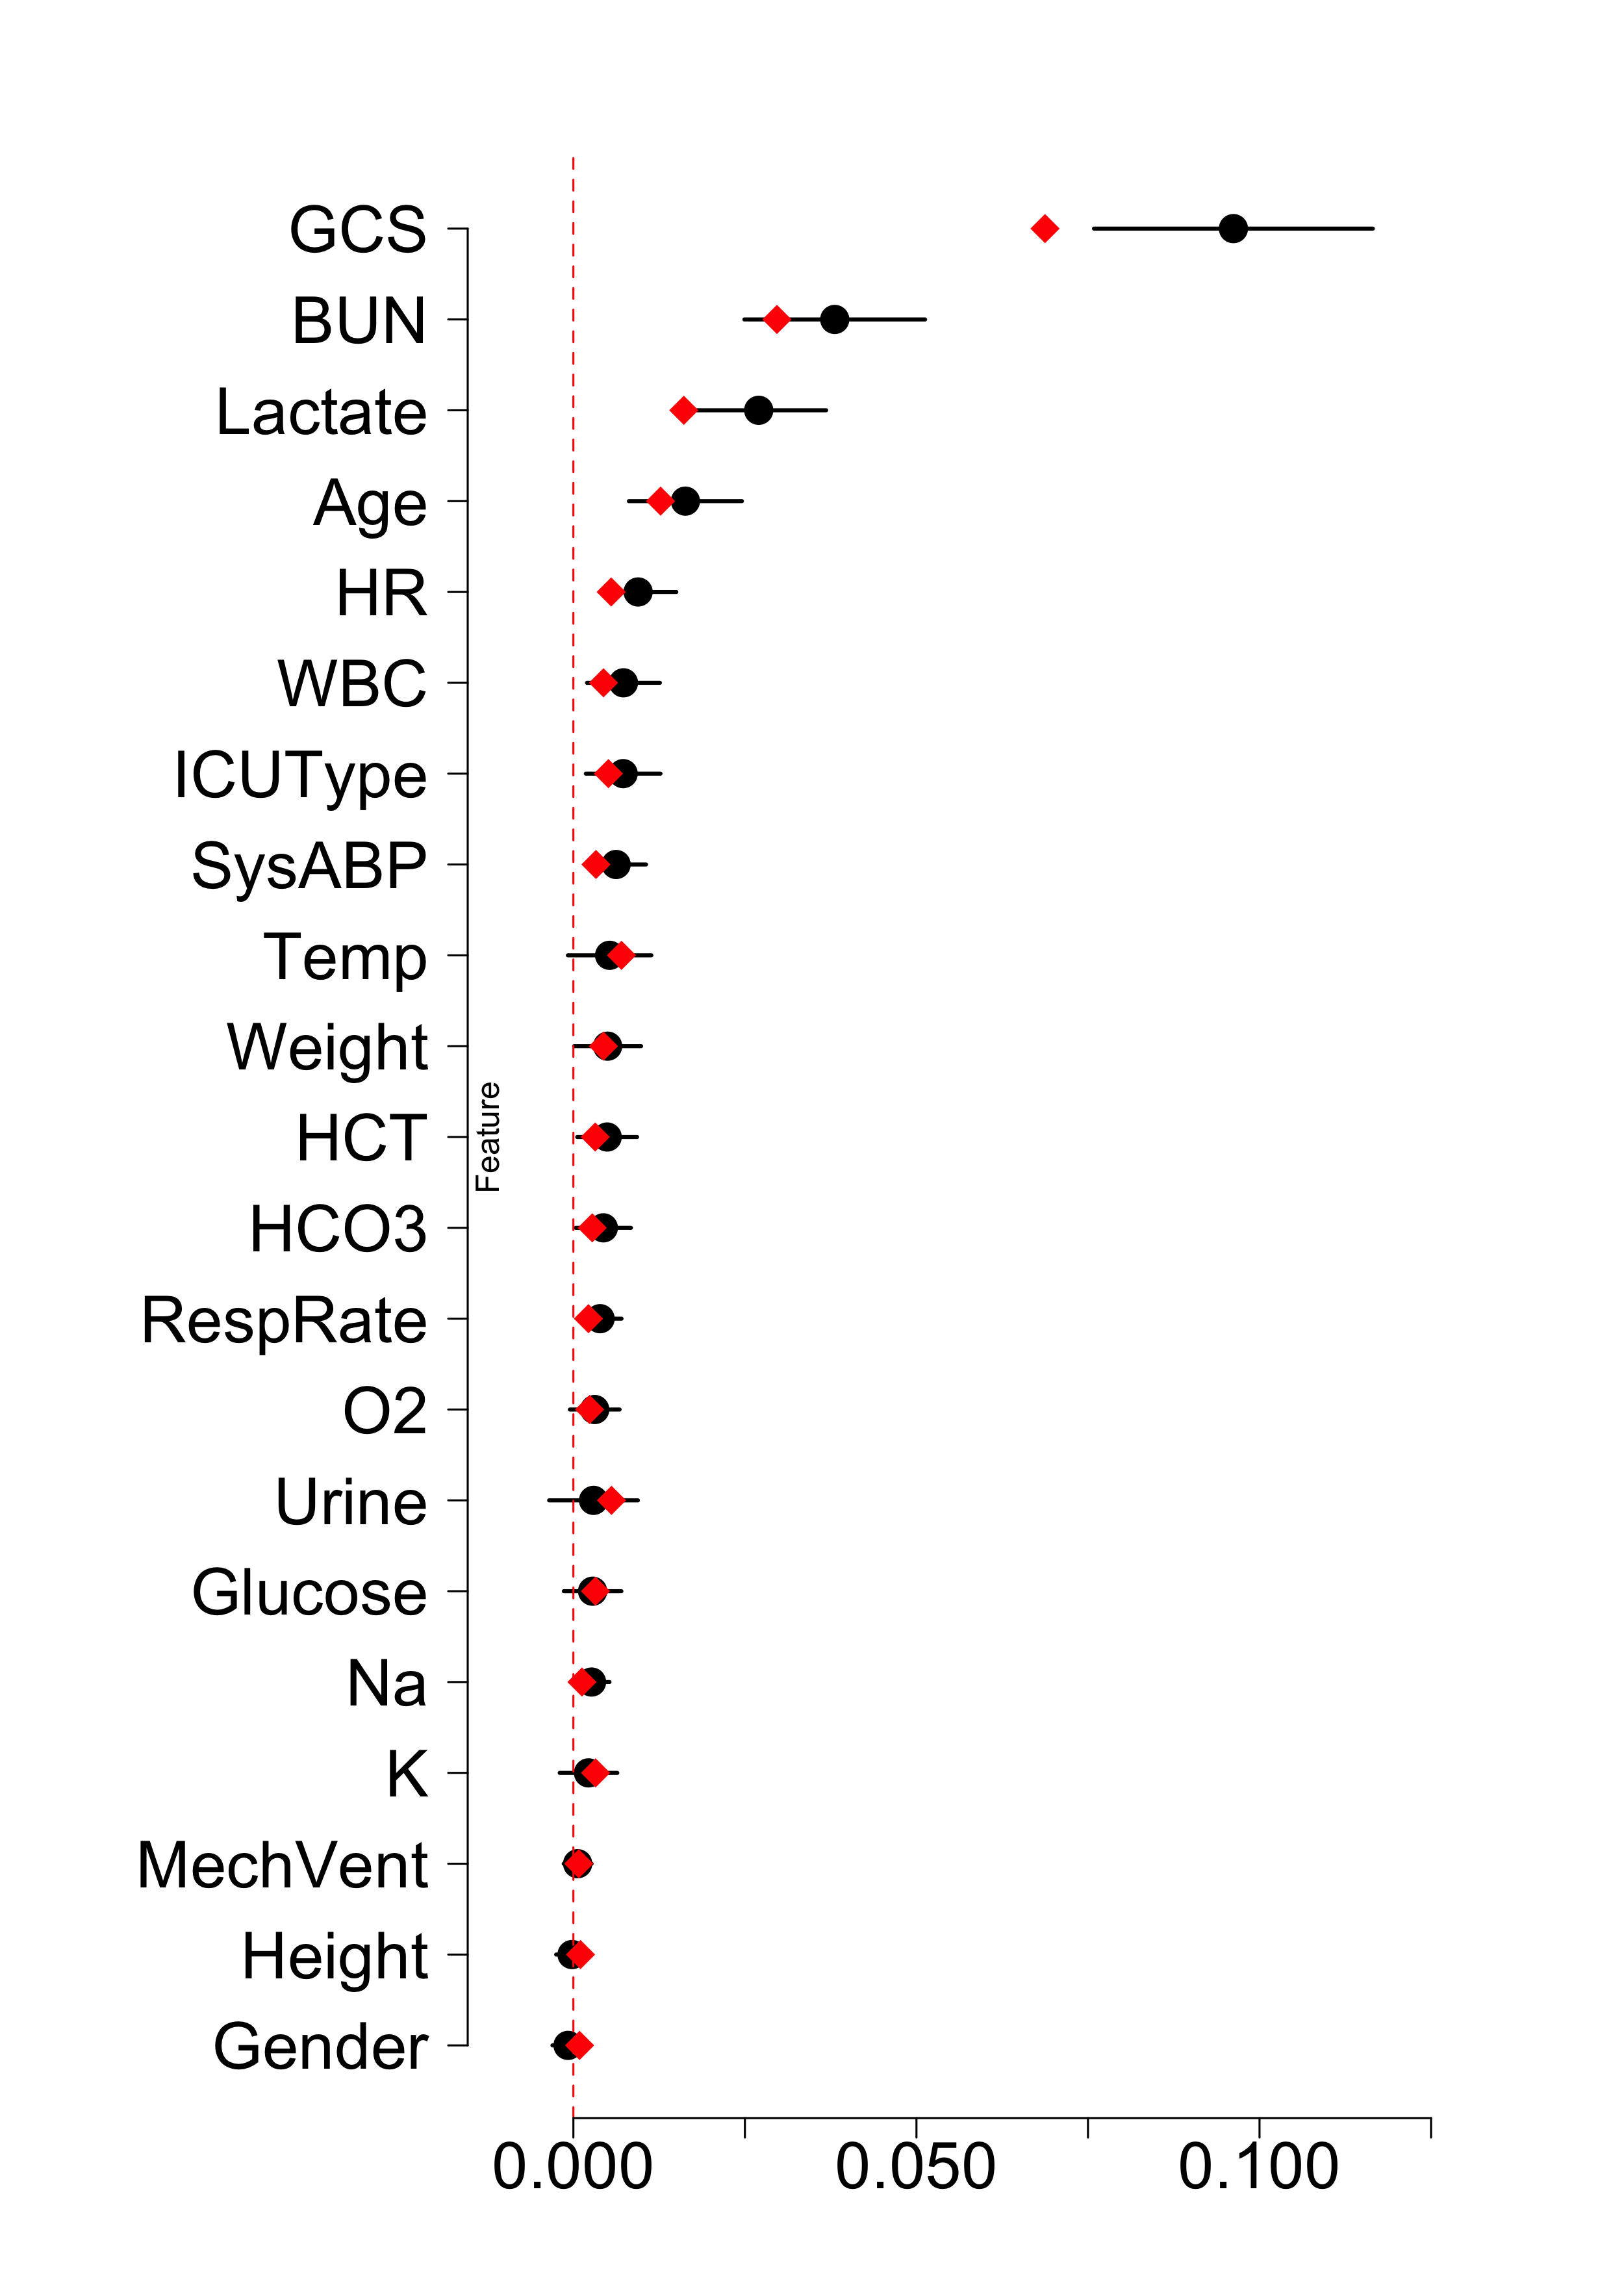
\includegraphics[width=0.4\textwidth]{images/icu_individual}
\caption{
	Variable importance estimates for tests in the ICU data (naive = red diamonds; corrected = black circles). Confidence intervals for the true importance, based on the corrected estimator only, are displayed as black bars.
}
\label{fig:icu_dat}
\end{figure}

Our method estimates that among the medical test variable groups, the Glasgow Coma Score test had the highest variable importance score by far (Figure~\ref{fig:icu_dat} top).
This makes sense as the Glasgow Coma Score scores the consciousness of a patient; the scoring system is based on whether the patient can open their eyes, talk, and move in response to various levels of stimuli.
Among all the medical tests, the GCS intuitively seems to have the most direct link to in-hospital mortality.
Our conclusion is also supported by the fact that GCS score can contribute the most number of points (up to 26 points) to the SAPS II score whereas most items in the SAPS II score contribute at most ~10 points.

The metabolic panel scored next highest in terms of variable importance.
This also makes sense as (1) this test is perhaps one of the most commonly ordered lab tests to assess patient health and (2) this test includes measurements of many different variables.
The primary driver of the importance of the metabolic test is blood urea nitrogen (BUN) which assesses kidney function.
Again, our conclusion is also supported by the SAPS II scoring method -- HCO3, BUN, Na, and K combined can contribute up to 24 points.

The confidence intervals for variable importance for urine and temperature include zero.
The low-importance of temperature makes sense -- temperature is one of the lowest-scoring items on SAPS II with a maximum contribution of 3 points.
Urine can contribute up to 11 points in SAPS II, but more modern mortality scoring methods like APACHE IV \citep{zimmerman2006acute} do not use urine output for predicting mortality.
As such, our results also suggest that to predict in-hospital mortality, we can drop measuring urine or temperature.
In fact, dropping urine measurements for mortality could relieve burden from patients and nurses; urine is typically quite taxing to monitor since (1) the patient must either be hooked up to a urine monitoring device (painful) or the patient must urinate into containers (annoying) and (2) the nurses must regularly measure the amount of urine over the course of a day.

%\section{Acknowledgments}
%for funders and people we like

\bibliography{paper.bib}
\bibliographystyle{icml2018}

\end{document}


% This document was modified from the file originally made available by
% Pat Langley and Andrea Danyluk for ICML-2K. This version was created
% by Iain Murray in 2018. It was modified from a version from Dan Roy in
% 2017, which was based on a version from Lise Getoor and Tobias
% Scheffer, which was slightly modified from the 2010 version by
% Thorsten Joachims & Johannes Fuernkranz, slightly modified from the
% 2009 version by Kiri Wagstaff and Sam Roweis's 2008 version, which is
% slightly modified from Prasad Tadepalli's 2007 version which is a
% lightly changed version of the previous year's version by Andrew
% Moore, which was in turn edited from those of Kristian Kersting and
% Codrina Lauth. Alex Smola contributed to the algorithmic style files.
